\section{Berechnung des Lenkwinkels}

Bekannt sind jetzt also der anzusteuernde Zielpunkt, die Pose des Roboters sowie dessen Radstand \gls{lat:radstand}. Anschließend soll der Zusammenhang zwischen Lenkwinkel und Zielpunkt hergeleitet werden. 
Aus der in Abb.~\ref{fig:regelung_prinzip_modell} dargestellten Geometrie lässt sich folgender Zusammenhang ablesen:

\begin{equation}
\tan \gls{gre:lenkwinkel} = \frac{\gls{lat:radstand}}{r_1}
\label{eq:regelung_lenkwinkel_lenkwinkeltan}
\end{equation}

Um einen Kreis eindeutig definieren zu können braucht man mindestens drei bekannte Parameter. Der noch unbekannte Radius \(r_1 = r\) lässt sich aus dem Zielpunkt, der Position und der Orientierung des Autos ausrechnen. Abbildung~\ref{fig:regelung_lenkwinkel_radius} zeigt eine anschauliche Möglichkeit zur Herleitung der gesuchten Beziehung. 

\begin{figure}[H] % [htb]
  \centering
  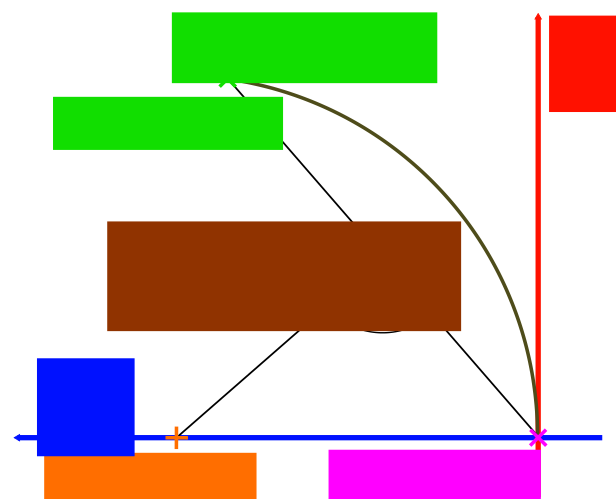
\includegraphics[width=0.8\textwidth]{regelung_lenkwinkel_radius.pdf}
  \caption{Veranschaulichung zur Bestimmung des Kreisradius aus dem gegebenen Zielpunkt in Roboterkoordinaten}
  \label{fig:regelung_lenkwinkel_radius}
\end{figure}

Es lassen sich zwei Hilfsgeraden \( g_1 \) und \( g_2 \) aufstellen. \(g_1\) verläuft durch die Position des Roboters \( p_0 \) und den Zielpunkt \( p_z \) und stellt somit die Sehne des Kreisbogens dar. Die Mittelsenkrechte dieser Sehne bildet die Gerade \( g_2 \).

\begin{eqnarray}
\text{Gerade }g_1: \quad y & = & m_z \cdot x 	\\
\text{Gerade }g_2: \quad y & = & m_h \cdot x + n_h  \label{eq:regelung_lenkwinkel_geradengleichung2}
\end{eqnarray}

Für den Schnittpunkt \( p_h \) gilt

\begin{eqnarray}
x_h & = & 0.5 \cdot x_z 	\\
y_h & = & 0.5 \cdot y_z
\end{eqnarray}

und für die Steigungen der Geraden gelten

\begin{eqnarray}
 m_z = \frac{\Delta y}{\Delta x} & = & \frac{y_z}{x_z} 	\\
 m_h = \frac{\Delta y}{\Delta x} & = & \frac{x_z}{-y_z}
\end{eqnarray}

Die \( y_{\gls{lat:RoboterKOS}} \)-Achse und die Gerade \( g_2 \) stehen jeweils senkrecht auf dem Kreisbogen und müssen sich demzufolge im Kreismittelpunkt \( p_M \) schneiden. Da \( p_M \) auf der \( y_{\gls{lat:RoboterKOS}} \)-Achse liegt ist die \( x_{\gls{lat:RoboterKOS}} \)-Koordinate mit \glqq 0\grqq{} bereits bekannt. Damit steht der gesuchte Radius in der \( y_{\gls{lat:RoboterKOS}} \)-Komponente des Mittelpunktes, was wiederum bedeutet, dass auch \( r = n_h \) gilt. Setzt man mit diesem Wissen den Punkt \( p_h \) in die Geradengleichung von \( g_2 \) (~\ref{eq:regelung_lenkwinkel_geradengleichung2}) ein, erhält man durch umstellen die Formel~\ref{eq:regelung_lenkwinkel_radius} für den Radius r.

\begin{equation}
r = n_h = y_h - m_h \cdot x_h = 0.5 \cdot \left( y_z + \frac{{x_z}^2}{y_z} \right)
\label{eq:regelung_lenkwinkel_radius}
\end{equation}

Ausgehend von Gleichung~\ref{eq:regelung_lenkwinkel_lenkwinkeltan} lässt sich nun der gesuchte Lenkwinkel mit Hilfe der Arcustangensfunktion bestimmen.

\begin{equation}
\gls{gre:lenkwinkel} = \arctan \left( \frac{\gls{lat:radstand}}{r} \right)
%\label{eq:regelung_lenkwinkel_lenkwinkel}
\end{equation}